\chapter{Mathematical Model of Vehicle Dynamics}

This chapter will detail the mathematical model that was developed to describe the motion of the uDrone. 

\section{Reference Frames and State Space}

Conventions for creating this model will follow those laid out by Thor Fossen in the 2011 Handbook of Marine Craft Hydrodynamics and Control. The fixed world frame is defined using the North-East-Down (NED) coordinate system, represented as $\{n\} = (x_n, y_n, z_n)$. in this system, $x_n$ points North, $y_n$ points East, and $z_n$ points down. 

The body-fixed frame $\{b\} = (x_b, y_b, z_b)$ is fixed its origin point, $o_b$, to the uDrone. For purposes of this model, $o_b$ is set at the point on the plane of the motors at the back of the uDrone that is along its center-line. $x_b$ runs along the center-line of the vehicle, pointing from the aft (back) of the uDrone to the fore (front). $z_b$ runs from top to bottom and, following the right-hand rule, $y_b$ runs towards the starboard (right). Further, following convention, roll is defined as rotation about $x_b$, pitch as rotation about $y_b$, and yaw as rotation about $z_b$, with counter-clockwise (CCW) being the positive direction. 

This choice of body frame origin reduces the complexity of modeling the forces produced by the motors. The drawback is some added complexity caused by the moments of the center of buoyancy and center of gravity relative to the chosen origin, but this is more straight forward than the complexity of calculating motor forces about a different point.

The position of the vehicle, or the body-fixed frame $\{b\}$, with respect to the world frame $\{n\}$ is expressed as $\bm{p} = [N, E, D]^T$. The attitude of the vehicle is expressed as $\bm{\Theta} = [\phi, \theta, \psi]^T$ using Euler angles. Together these create the 6-dimensional position/orientation vector $\bm{\eta} = [\bm{p}, \bm{\Theta]}^T$. The linear and angular velocities are expressed with respect to the vehicles fixed frame $\{b\}$. The linear velocity is $\bm{v} = [u, v, w]^T$ and angular velocity $\bm{\omega} = [p, q, r]^T$. when combine, these form the combine 6-dimensional velocity vector $\bm{\nu}= [\bm{v}, \bm{\omega]}^T$. All together, $\boldsymbol{\eta}$ and $\boldsymbol{\nu}$ represent the 12-dimensional state space describing the state of the uDrone \parencite{thor_kin}. 

% \begin{align*}
%      \boldsymbol{p}^{n}_{b}=\left[\begin{array}{c}
%         N \\ E \\ D
%      \end{array}\right]
%      \bm{\Theta}^{n}_{b}=\left[\begin{array}{c}
%         \phi \\ \theta \\ \psi
%      \end{array}\right]
%      \bm{\eta}=\left[\begin{array}{c}
%         \bm{p} \\ \bm{\Theta}
%      \end{array}\right]
% \end{align*}
% \begin{align*}
%      \boldsymbol{v}^{b}_{b}=\left[\begin{array}{c}
%         u \\ v \\ w
%      \end{array}\right]
%      \bm{\omega}^{b}_{b}=\left[\begin{array}{c}
%         p \\ q \\ r
%      \end{array}\right]
%      \bm{\nu}=\left[\begin{array}{c}
%         \bm{v} \\ \bm{\omega}
%      \end{array}\right]
% \end{align*}



\section{Equations of Motions}

The general equation of motion for the uDrone can be derived as a function of the combine linear and angular velocity vector $\boldsymbol{\nu}$ \parencite{thor_mod}. This is shown in equation \ref{eqm}.

\begin{gather}
\underbrace{\boldsymbol{M}_{R B} \dot{\boldsymbol{\nu}}+\boldsymbol{C}_{R B}(\boldsymbol{\nu}) \boldsymbol{\nu}}_{\text {rigid-body forces}}+\underbrace{\boldsymbol{M}_{A} \dot{\boldsymbol{\nu}}+\boldsymbol{C}_{A}\left(\boldsymbol{\nu}\right) \boldsymbol{\nu}+\boldsymbol{D}\left(\boldsymbol{\nu}\right) \boldsymbol{\nu}}_{\text {hydrodynamic forces}}+\underbrace{\boldsymbol{g}(\boldsymbol{\eta})}_{\text{hydrostatic forces}}=\boldsymbol{\tau}
\label{eqm}
\end{gather}
With the terms defined as:
\begin{align*}
    \boldsymbol{\eta}&=\text{combine position and orientation}\\
    \boldsymbol{\nu}&=\text{combine linear and angular velocity}\\
    \dot{\boldsymbol{\nu}}&=\text{combine linear and angular acceleration}\\
    \boldsymbol{M}_{R B}&=\text{rigid-body system inertia matrix}\\
    \boldsymbol{C}_{R B}(\boldsymbol{\nu})&=\text{rigid-body Coriolis matrix}\\
    \boldsymbol{M}_{A}&=\text{added mass system inertia matrix}\\
    \boldsymbol{C}_{A}(\boldsymbol{\nu})&=\text{added mass Coriolis matrix}\\
    \boldsymbol{D}(\boldsymbol{\nu})&=\text{damping matrix}\\
    \boldsymbol{g}(\boldsymbol{\eta})&=\text{gravitational and buoyant forces}\\
    \boldsymbol{\tau}&=\text{control inputs}
\end{align*}
% \begin{align*}
%     \boldsymbol{\eta}&=\text{combine position and orientation}\\
%     \boldsymbol{\nu}&=\text{combine linear and angular velocity}\\
%     \dot{\boldsymbol{\nu}}&=\text{combine linear and angular acceleration}\\
%     \boldsymbol{\tau}&=\text{control inputs}\\
%     \boldsymbol{M}&=\text{system inertia matrix}\\
%     \boldsymbol{C}(\boldsymbol{\nu})&=\text{Coriolis matrix}\\
%     \boldsymbol{D}(\boldsymbol{\nu})&=\text{damping matrix}\\
%     \boldsymbol{g}(\boldsymbol{\eta})&=\text{gravitational and buoyant forces}\\
%     \boldsymbol{\tau}&=\text{control inputs}
% \end{align*}
% \begin{align*}
%     \boldsymbol{M}&=\boldsymbol{M}_{R B}+\boldsymbol{M}_{A}\\
%     \boldsymbol{C}&=\boldsymbol{C}_{R B}+\boldsymbol{C}_{A}
% \end{align*}

\section{Rigid-Body Forces}

The exact values of the system inertia ($\boldsymbol{M}$), Coriolis ($\boldsymbol{C}$), and Drag ($\boldsymbol{D}$) matrices can be determined either through intensive hydrodynamic modeling or experimentation. Due to the complexity of hydrodynamic modeling, experimentation is typically used to determine these values in underwater vehicles similar to the uDrone \parencite{hipp_pen}. It is possible, however, to estimate the rigid body matrix values using information about the vehicle generated from the 3D model. This section details these estimations and explains how they were calculated. 

The rigid body system inertia matrix about the center of origin can be calculated using equation \ref{mrb} which is found in \cite{thor_rb}.
\begin{gather}
    \boldsymbol{M}_{R B}^{C O}=\left[\begin{array}{cc}
        m \boldsymbol{I}_{3 \times 3} & -m \boldsymbol{S}\left(\boldsymbol{r}_{g}^{b}\right) \\
        m \boldsymbol{S}\left(\boldsymbol{r}_{g}^{b}\right) & \boldsymbol{I}_{g}-m \boldsymbol{S}^{2}\left(\boldsymbol{r}_{g}^{b}\right)
    \end{array}\right]
    \label{mrb}
\end{gather}
% \begin{align*}
%     \boldsymbol{M}_{R B}^{C O}&=\text{rigid body system inertia matrix about the body fixed-frame origin}\\
%     \boldsymbol{I}_{3 \times 3}&=\text{3 by 3 identity matrix}\\
%     m&=\text{mass}\\
%     \boldsymbol{S}(\cdot)&=\text{cross product operator}\\
%     \boldsymbol{r}_{g}^{b}&=\text{ vector from the body fixed-frame origin to the center of gravity}\\
%     \boldsymbol{I}_{g}&=\text{inertia matrix}
% \end{align*}

In this equation, $m$ is the mass, $\boldsymbol{I}_{3 \times 3}$ is the three-by-three identity matrix, $\boldsymbol{I}_{g}$ is the inertia matrix and $\boldsymbol{r}_{g}^{b}$ is the vector from the body fixed-frame origin to the center of gravity. $\boldsymbol{S}$ is the cross product operator matrix. Before the final vehicle was constructed, m, $\boldsymbol{I}_{g}$, and $\boldsymbol{r}_{g}^{b}$ were taken from the 3D model. Those estimates are shown in equation \ref{m_matrix}.

\begin{equation}
\boldsymbol{M}_{R B}^{C O}=\left[\begin{array}{cccccc}
9.9000 & 0 & 0 & 0 & 0 & 0 \\
0 & 9.9000 & 0 & 0 & 0 & 1.4850 \\
0 & 0 & 9.9000 & 0 & -1.4850 & 0 \\
0 & 0 & 0 & 0.3420 & 0.0010 & -0.0001 \\
0 & 0 & -1.4850 & 0.0010 & 0.5577 & -0.0015 \\
0 & 1.4850 & 0 & -0.0001 & -0.0015 & 0.3167
\end{array}\right]
\label{m_matrix}
\end{equation}


With a completed vehicle these numbers can be verified and varied if needed. For example, with no ballast, the uDrone is positively buoyant. Therefore, to maintain its depth without using power to stay underwater ballast will need to be added. By placing the ballast closer to the center of the vehicle, the moments of inertia will decrease. Conversely, by placing it further from the center the moments can be increased. Additionally, the ballast can be used to change the center of gravity relative to the center of buoyancy. This will create a moment in the vehicle that can help it stay oriented or level in specific ways. This relationship is discussed further in the section \ref{hydrostatics}. 

The Coriolis matrix is a function of the angular velocity of the vehicle and can be derived as shown in equation \ref{crb} from \cite{thor_rb}.
\begin{gather}
    \boldsymbol{C}_{RB}^{CO}(\boldsymbol{\nu})=\left[\begin{array}{cc}
        m \boldsymbol{S}\left(\boldsymbol{\omega}^{b}\right) & -m \boldsymbol{S}\left(\boldsymbol{\omega}^{b}\right) \boldsymbol{S}\left(\boldsymbol{r}_{g}^{b}\right) \\
        m \boldsymbol{S}\left(\boldsymbol{r}_{g}^{b}\right) \boldsymbol{S}\left(\boldsymbol{\omega}^{b}\right) & -\boldsymbol{S}\left(\left(\boldsymbol{I}_{g}-m \boldsymbol{S}^{2}\left(\boldsymbol{r}_{g}^{b}\right)\right) \boldsymbol{\omega}^{b}\right)
    \end{array}\right]
    \label{crb}
\end{gather}
% \begin{align*}
%     \boldsymbol{C}_{R B}^{C O}&=\text{rigid body Coriolis matrix about the body fixed-frame origin}\\
%     m&=\text{mass}\\
%     \boldsymbol{S}(\cdot)&=\text{cross product operator}\\
%     \boldsymbol{\omega}^b&=\text{body-fixed frame angular velocity}\\
%     \boldsymbol{r}_{g}^{b}&=\text{ vector from the body fixed-frame origin to the center of gravity}\\
%     \boldsymbol{I}_{g}&=\text{inertia matrix}
% \end{align*}

Where $\boldsymbol{\omega}^{b}$ is the body-fixed frame angular velocity vector. Since this matrix is a function of the vehicle state, it will change with motion. The actual calculations of this matrix are handled by a MatLab program written as a companion to Thor Forson’s book \parencite{mss}. The values based on the system inertia matrix in equation \ref{m_matrix} along with a velocity state vector $\bm{\nu}= [1,0,0,0,0,0]^T$, which represents only forward motion, is shown in equation \ref{c_matrix}.

\begin{equation}
\boldsymbol{C}_{RB}^{CO}(\boldsymbol{\nu})=\left[\begin{array}{cccccc}
0 & 0 & 0 & 0 & 0 & 0 \\
0 & 0 & 0 & 0 & 0 & 9.9000 \\
0 & 0 & 0 & 0 & -9.9000 & 0 \\
0 & 0 & 0 & 0 & 0 & 0 \\
0 & 0 & 9.9000 & 0 & 0 & 0 \\
0 & -9.9000 & 0 & 0 & 0 & 0
\end{array}\right]
\label{c_matrix}
\end{equation}

\section{Hydrostatic Forces} \label{hydrostatics}

The hydrostatic term $\boldsymbol{g}(\boldsymbol{\eta})$ accounts for the forces on the uDrone caused by gravity and buoyancy. The force of gravity, or weight ($W$) is equal to the mass of the uDrone times the acceleration due to gravity. The buoyant force ($B$) is the weight of the water displaced by the uDrone. This is calculated by multiplying the volume of the uDrone, the density of water, and the acceleration due to gravity. If the location of the center of gravity and center of buoyancy (or center of volume) of the uDrone are not in the same spot then there will be a moment on the whole vehicle. Similarly, if the two forces are not equal then there will also be a net linear force on it. This value is a function of the orientation of the vehicle and can be seen in equation \ref{bigG} \parencite{thor_rb}. 

\begin{equation}\label{bigG}
\boldsymbol{g}(\boldsymbol{\eta})=\left[\begin{array}{llll} 
& (W-B) \sin (\theta) \\
- & (W-B) \cos (\theta) \sin (\phi) \\
- & (W-B) \cos (\theta) \cos (\phi) \\
- & \left(y_{g} W-y_{b} B\right) \cos (\theta) \cos (\phi) & + & \left(z_{g} W-z_{b} B\right) \cos (\theta) \sin (\phi) \\
& \left(z_{g} W-z_{b} B\right) \sin (\theta) & + & \left(x_{g} W-x_{b} B\right) \cos (\theta) \cos (\phi) \\
- & \left(x_{g} W-x_{b} B\right) \cos (\theta) \sin (\phi) & - & \left(y_{g} W-y_{b} B\right) \sin (\theta)
\end{array}\right]
\end{equation}

% \begin{equation}
%   \boldsymbol{g}(\boldsymbol{\eta})=\left[\begin{array}{llll}  
%   0\\0\\0\\0\\0\\0
%   \end{array}\right]
% \end{equation}

Ballasting can be used to adjust the weight and center of mass on the uDrone. To simplify this equation the ballast is set so that the weight and buoyancy are equal and the center of mass and buoyancy are the same. This means the $\boldsymbol{g}$ vector will be zeros for all $\boldsymbol{\eta}$. These forces can be seen interacting on the uDrone in figure \ref{cord_frame}. Maintaining overlapped centers of buoyancy and gravity also makes the vehicle more nimble as there are less moments to overcome when rotating. This also has the benefit of making the uDrone more maneuverable. Equal weight and buoyancy reduces energy used as the uDrone does not need to overcome a force making it sink or float as it cruises through the water column. 

There might be reasons to adjust the ballasting of the uDrone to impart other properties on it. For example, if the vehicle is slightly positively buoyant than it will float in the event of a power failure, allowing for it to be recovered more easily. Also, if the center of gravity is placed below the center of buoyancy, but still in line with it in the z body direction, then the vehicle will be self righting in roll. This could make control easier as roll, which should be at zero most of the time, can be ignored.

\section{Hydrodynamic Forces} \label{hydrodynamics}

The added mass system inertia matrix and added mass Coriolis matrix can only be determined through experimentation or complex fluid dynamic simulation and are not calculated in the scope of this thesis. The damping matrix, however, can be estimated using drag calculations. 

The vehicle is modeled as a flat-faced cylinder moving through water in a direction along its axis. This estimation neglects two factors: 1) drag from the motors, and 2) rotational damping. Both of these forces are small in comparison to the drag of the flat-faced cylinder, so for the purposes of an approximate model, they can be ignored. 

The force of drag in a single direction can be calculated using the drag equation:

\begin{gather}
F_{D}=C_{D} A \frac{\rho V^{2}}{2}
\end{gather}
\begin{align*}
    F_D&=\text{drag Force}\\
    C_D&=\text{coefficient of drag}\\
    A&=\text{cross-sectional area normal to velocity}\\
    \rho&=\text{fluid density}\\
    V&=\text{velocity}\\
\end{align*}

Based on the ratio of the diameter to the length of the main body of the uDrone, the Coefficient of drag in the direction of motion is estimated at 0.8. The density of salt water is 1024kg/m$^3$ and the surface area is calculated from the diameter of the eight inch cylinder, which is 0.037m$^2$. Putting this all together, damping force can be calculated as a function of velocity. This is:

\begin{gather}
    \boldsymbol{D}(\boldsymbol{\nu})\boldsymbol{\nu}=\left[\begin{array}{c}
        -15.0u ^2 \\ \sim 0 \\ \sim 0 \\ D_{roll} \\ D_{pitch} \\ D_{yaw}
     \end{array}\right]
\end{gather}

$u$ is the velocity in the x body direction. The last three values which refer to the rotational damping. For the purposes of calculations in the next section these values were assumed to be zero. The second and third terms, however, will always be zero, or nearly zero, as the vehicle cannot independently move in the Y or Z direction.

\section{Control Inputs}\label{control_inputs}

The control inputs are the forces put on the uDrone from the thrusters. The four motor of the uDrone are arranged on a plane, all facing the same direction. The center point between all the thrusters along that plane is the Center of Origin $C_O$ for the vehicle. Thrusters one and three spin in a counterclockwise direction while thrusters two and four spin clockwise for forward thrust. This ensures that the vehicle has no roll moment when moving forward. Figure \ref{cord_frame} shows the uDrone with the $C_O$ and rotation direction of the thrusters. 

\begin{figure}[h]
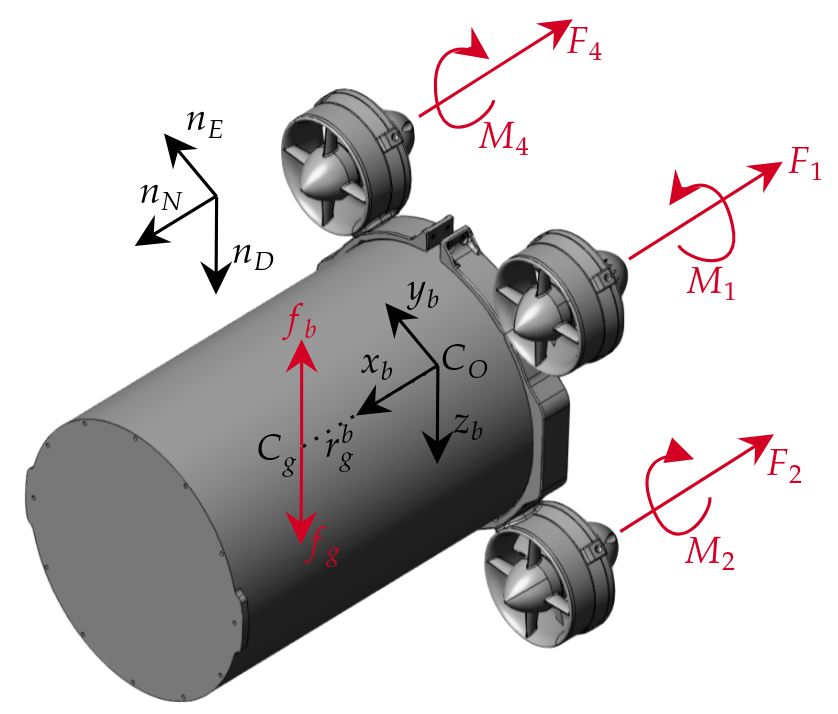
\includegraphics[width=\maxwidth{\textwidth}]{img/cord_frame.png}
\caption{uDrone Coordinate Frame and Motor Directions}
\label{cord_frame}
\end{figure}

Using this convention it is possible to determine the actuation matrix, tau, as a function of thruster inputs.

\begin{gather}
    \boldsymbol{\tau}=\left[\begin{array}{c}
        F_1+F_2+F_3+F_4 \\ 0 \\ 0 \\ M_1-M_2+M_3-M_4 \\ (F_2+F_3-F_1-F_4) \frac{L}{\sqrt{2}} \\ (F_1+F_2-F_3-F_4) \frac{L}{\sqrt{2}}
     \end{array}\right]
     \label{tau}
\end{gather}

In equation \ref{tau} $F_x$ indicates the linear force produced by the $x^{th}$ motor and $M_x$ indicates the angular momentum produced by the $x^{th}$. $L$ is 0.115m, the length from $C_O$ to the center of the motor, which is the same for each motor. Unfortunately, there is no data from Blue Robotics about the moment of the thrusters, so the relationship between control input to the roll moment will need to be determined experimentally. Data is available, however, correlating motor power and thrust force. 

\begin{figure}[h]
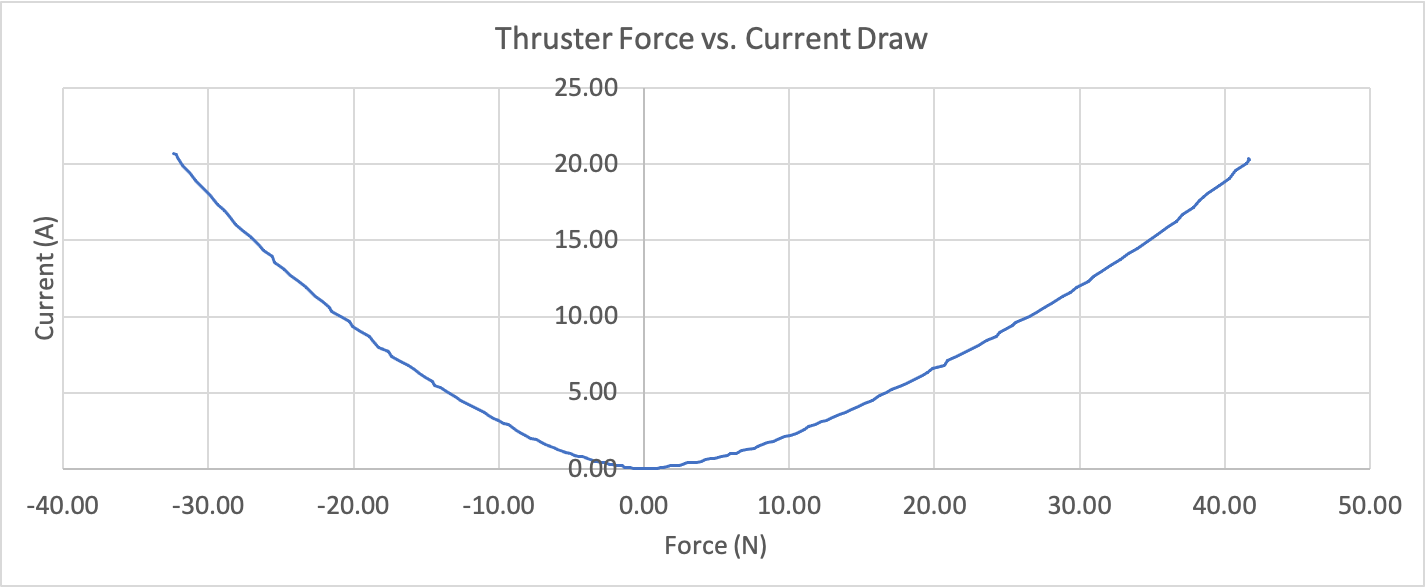
\includegraphics[width=\maxwidth{\textwidth}]{img/force_amps.png}
\caption{Force Output vs. Current Draw for T200 Thruster at 14 Volts}
\label{force_amp}
\legend{\emph{Source}: \iftoggle{usebiblatex}{\textcite{t200}}{\citet{t200}}}% See: https://upload.wikimedia.org/wikipedia/commons/8/89/Antidorcas_marsupialis%2C_male_%28Etosha%2C_2012%29.jpg
% \legend{\emph{Note}: Here is a note that is especially long to show what happens when it extends to more than one line.}
\end{figure}


Using the figure \ref{force_amp}, along with data about the uDrone battery, it is possible to calculate the maximum velocity, running time at this velocity, and running time at the operational velocity of 1m/s. While the uDrone can carry two 14V, 18Ah batteries, the intent is to use one for thrusters and the other to control all electronics. Therefore, all longevity calculations are done assuming 18Ah are available for thruster actuation. 

In order to calculate maximum velocity, the drag equation is set equal to the maximum thruster force. The T200 thrusters produce a maximum thrust of 41.68N each. This is 166.7N of total thrust. Setting this equal to $15u^2$ and solving yields a maximum speed of 3.33m/s. Maintaining this velocity takes 20.29A, for a total of 81.16A. The uDrone could only maintain this speed for approximately 13.3 minute with an 18Ah battery.

Typically, however, the uDrone will be cruising at a speed of 1m/s. At this speed, the drag force is approximately 15N. To maintain this thrust each motor must produce about 3.75N of force. To maintain this force each motor will use approximately 0.5A, for a total of 2A. In order to stay conservative, a 50\% safety factor will be added to this value to account for uncalculated drag forces and actuation that affect orientations, not just forward motion. With this addition, the vehicle will use 3A for actuation during normal operation. With a single 18Ah battery used for thrusters, this will yield a dive time of approximately 6 hours. 
